\chapter{Metodologia} \label{cap4}
Este capítulo apresenta as técnicas e o protocolo experimental utilizados para a construção e avaliação dos modelos preditivos. Sua organização segue as etapas do processo de descoberta de conhecimento em bases de dados.

\section{Base de Dados}

Neste projeto foi utilizado o Indian Liver Patient Dataset (ILPD) \cite{ramana2022ilpd}, 
um dataset de 583 registros contendo dados bioquímicos relacionados ao fígado, 
visando auxiliar na predição de patologias hepáticas. O dataset é composto por 10 atributos, 
sendo 9 variáveis bioquímicas e 1 variável demográfica, além da variável-alvo que classifica 
os pacientes em diagnosticados com doença hepática ou sem esse diagnóstico.

\subsection{Caracterização das Variáveis}

O conjunto de dados contém as seguintes variáveis preditoras:

\begin{enumerate}
    \item \textbf{Age}: idade do paciente em anos (numérica);
    \item \textbf{Gender}: sexo do paciente, codificado como Male ou Female (categórica);
    \item \textbf{Total\_Bilirubin}: concentração de bilirrubina total em mg/dL (numérica);
    \item \textbf{Direct\_Bilirubin}: concentração de bilirrubina direta em mg/dL (numérica);
    \item \textbf{Alkaline\_Phosphotase}: atividade de fosfatase alcalina em IU/L (numérica);
    \item \textbf{Alamine\_Aminotransferase}: atividade de alanina aminotransferase (ALT/TGP) em IU/L (numérica);
    \item \textbf{Aspartate\_Aminotransferase}: atividade de aspartato aminotransferase (AST/TGO) em IU/L (numérica);
    \item \textbf{Total\_Proteins}: concentração de proteínas totais em g/dL (numérica);
    \item \textbf{Albumin}: concentração de albumina em g/dL (numérica);
    \item \textbf{AG\_Ratio}: razão albumina/globulina (numérica).
\end{enumerate}

A variável-alvo é binária, classificando os pacientes como portadores de doença hepática 
(\textit{Dataset} = 1) ou não (\textit{Dataset} = 2), conforme diagnóstico clínico 
estabelecido no momento da coleta. Cabe uma ressalva sobre o significado da segunda 
classe: o rótulo \textit{Dataset} = 2 indica apenas que o paciente \textbf{não recebeu 
diagnóstico de doença hepática} no momento da coleta, e não que ele seja comprovadamente 
saudável. Essa distinção é relevante porque todos os indivíduos da base passaram por 
exames laboratoriais hepáticos, o que sugere que havia alguma suspeita clínica inicial 
mesmo nos casos sem diagnóstico confirmado. Ao longo deste trabalho, por simplicidade 
de redação, os pacientes com \textit{Dataset} = 2 serão chamados de ``saudáveis'' ou 
``não doentes'', mas o leitor deve ter em mente que o termo se refere à ausência de 
diagnóstico registrado, e não a um estado de saúde verificado.

\subsection{Distribuição das Classes e Desbalanceamento}

O dataset apresenta desbalanceamento significativo de classes. Dos 583 registros originais, 
416 pacientes (71,4\%) foram classificados como doentes hepáticos, enquanto 167 pacientes 
(28,6\%) foram classificados como saudáveis, resultando em uma razão de aproximadamente 
2,5:1 entre as classes. Essa distribuição desigual impõe desafios na modelagem, pois 
classificadores ingênuos poderiam atingir alta acurácia simplesmente predizendo todos os 
pacientes como doentes, sem capturar informações discriminativas reais.

\subsection{Contexto e Limitações}

Os dados foram coletados em pacientes do nordeste de Andhra Pradesh, Índia, representando 
uma população geograficamente circunscrita. A caracterização clínica de ``doença hepática'' 
no dataset é agregada, não diferenciando entre diferentes patologias hepáticas (hepatite, 
cirrose, esteatose, etc.). Além disso, a base contém apenas 4 valores ausentes na variável 
\textit{AG\_Ratio} e 13 registros duplicados, indicando qualidade geral satisfatória dos dados.

O ILPD é um dataset amplamente utilizado na literatura de aprendizado de máquina aplicado 
ao diagnóstico médico \cite{ramana2022ilpd}, permitindo comparação com estudos anteriores. 
Contudo, seu tamanho reduzido (583 pacientes) e sua origem em uma população específica 
limitam a generalização dos resultados para outras populações e contextos clínicos.

\section{Análise Exploratória de Dados}

Antes de qualquer transformação dos dados ou do treinamento de modelos, foi feita 
uma Análise Exploratória de Dados (AED). A AED é uma etapa importante em qualquer 
projeto de aprendizado de máquina, porque permite entender a estrutura, a qualidade 
e o comportamento estatístico das variáveis antes de se tomar decisões de modelagem 
\cite{exploratorydataanalysis}. 
As decisões de pré-processamento descritas nas próximas seções, como a remoção de 
duplicatas, a transformação logarítmica e a imputação de valores ausentes, foram 
tomadas com base no que esta análise revelou, e não definidas \textit{a priori}.

É importante ressaltar que a AED foi feita sobre o conjunto completo de dados, com finalidade 
\textbf{apenas descritiva}. Nenhum parâmetro calculado nesta etapa (médias, medianas, 
desvios-padrão) foi usado para transformar os dados que alimentam os modelos. Esses 
parâmetros são estimados somente no conjunto de treino, depois da divisão treino/teste, 
como explicado na seção seguinte. Esse cuidado evita o chamado \textit{vazamento de 
dados} (\textit{data leakage}), em que informações do conjunto de teste contaminam o 
treinamento e levam a estimativas de desempenho otimistas demais \cite{KaufmanScharRosset2012, KAPOOR2023100804}.

Toda a análise foi implementada na linguagem R \cite{linguagemr}, com os pacotes 
\texttt{tidyverse} \cite{tidyverse} para manipulação e visualização dos dados e 
\texttt{corrplot} \cite{corrplot2024} para a visualização das matrizes de correlação. 
Usou-se uma semente aleatória fixa ao longo de todo o \textit{pipeline}, para 
garantir a reprodutibilidade dos resultados \cite{Pineau2020Improving}.

As etapas da análise exploratória são descritas a seguir.

\subsection{Leitura e Verificação Estrutural}

O arquivo original do ILPD é distribuído em formato CSV sem cabeçalho. Por isso, os 
nomes das colunas foram atribuídos manualmente na leitura, seguindo a documentação 
oficial do repositório UCI \cite{ramana2022ilpd}. Depois da leitura, conferiu-se 
que o número de observações (583) e de atributos (11, contando a variável-alvo) 
correspondia ao documentado, e verificou-se o tipo de cada variável. Essa conferência 
garante que nenhuma coluna foi lida com tipo errado, como uma variável numérica 
interpretada como texto por causa de um caractere inválido. Erros desse tipo passariam 
despercebidos e comprometeriam todas as etapas seguintes.

\subsection{Valores Ausentes}

Contou-se a quantidade de valores ausentes em cada variável. Apenas o atributo 
\textit{AG\_Ratio} apresentou dados faltantes: 4 registros, cerca de 0,69\% da base. 
Como a proporção é muito pequena, descartaram-se as alternativas mais agressivas, 
como excluir a variável ou usar métodos de imputação mais complexos (imputação 
múltipla, imputação por $k$ vizinhos mais próximos). Optou-se pela imputação pela 
\textbf{mediana}. A mediana é preferível à média porque é uma medida de tendência 
central robusta, pouco afetada pelos valores extremos e pela assimetria típicos de 
dados laboratoriais \cite{batistamonard2003}.

Com uma quantidade tão pequena de ausências, é razoável supor que o método de 
imputação tem impacto desprezível nos resultados \cite{acunaedgar}.

\subsection{Registros Duplicados}

Foram encontrados 13 registros exatamente duplicados, isto é, linhas idênticas em 
todos os atributos, inclusive na variável-alvo. Nesta etapa exploratória eles foram 
apenas identificados e mantidos, para que as estatísticas descritivas refletissem a 
base original tal como é distribuída.

A remoção desses registros, feita na etapa de pré-processamento, é importante por 
dois motivos. O primeiro é que registros duplicados 
podem acabar um no conjunto de treino e outro, idêntico, no conjunto de teste. 
Nesse caso o modelo é avaliado em exemplos que já "viu" durante o treinamento, o 
que infla artificialmente as métricas de desempenho \cite{KAPOOR2023100804}. O segundo é que 
duplicatas dão peso desproporcional a certos padrões, distorcendo a distribuição 
aprendida pelo modelo\cite{christenpeter2012}. Como a base não traz identificadores de paciente, não é 
possível saber se as duplicatas são erros de registro ou pacientes distintos com 
exames coincidentes. Mesmo assim, a coincidência exata em dez atributos contínuos 
torna a segunda hipótese pouco provável.

\subsection{Distribuição da Variável-Alvo e do Sexo}

Calculou-se a frequência absoluta e relativa de cada classe da variável-alvo, o que 
confirmou a razão de desbalanceamento de cerca de 2,5:1 descrita anteriormente 
(Figura~\ref{fig:eda_distribuicao_alvo}). Esse diagnóstico justificou duas decisões metodológicas. 
A primeira foi usar \textbf{divisão estratificada} entre treino e teste, que preserva a mesma 
proporção de classes nos dois conjuntos, detalhada na Seção~\ref{sec:divisao_treino_teste}. 
A segunda foi aplicar técnicas de balanceamento apenas no conjunto de treino, detalhada na 
Seção~\ref{sec:balanceamento}. O diagnóstico também justificou o uso
de métricas menos sensíveis ao desbalanceamento do que a acurácia, como a área sob 
a curva ROC (AUC), a sensibilidade e a especificidade \cite{FAWCETT2006861, imbalancedata}.

\begin{figure}[htbp]
\centering
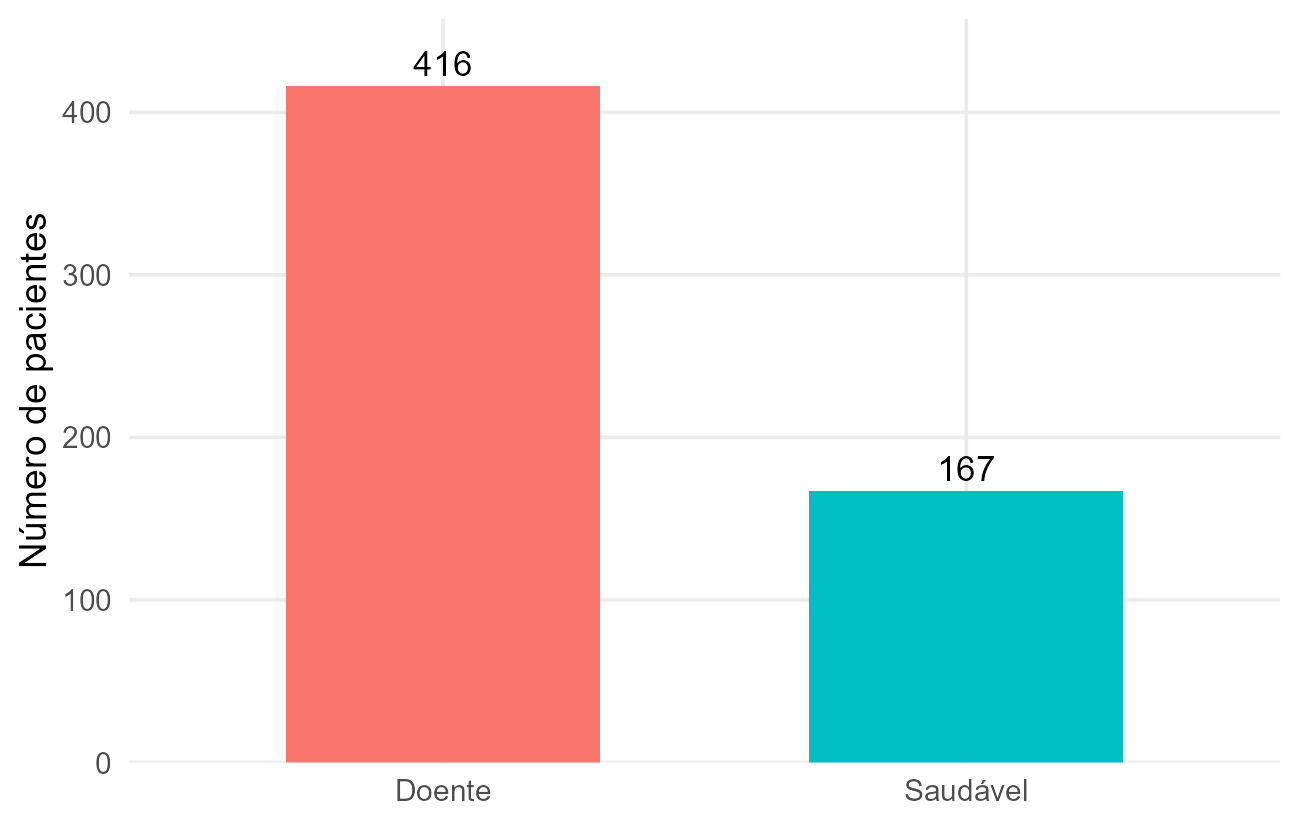
\includegraphics[width=0.7\textwidth]{figuras/cap4-metodologia/eda_distribuicao_alvo.png}
\caption{Distribuição da variável-alvo (doentes \textit{vs.} saudáveis).}
\label{fig:eda_distribuicao_alvo}
\end{figure}

Também se construiu uma tabela de contingência entre o sexo do paciente e a 
variável-alvo. A base é composta majoritariamente por pacientes do sexo masculino 
(cerca de 76\%). Esse desequilíbrio é relevante para o objetivo de interpretabilidade 
deste trabalho: se um grupo demográfico está sub-representado, o modelo pode ter 
desempenho desigual entre os grupos e aprender relações enviesadas \cite{Rajkomar2018Ensuring, investigatingbiashealth}. Por esse 
motivo, a avaliação dos modelos e a análise de interpretabilidade foram feitas também 
de forma estratificada por sexo.

\subsection{Estatísticas Descritivas e Assimetria}
\label{sec:estatisticas_descritivas_assimetria}

Para cada uma das nove variáveis numéricas foram calculadas a média, o 
desvio-padrão, o mínimo, a mediana, o máximo e o coeficiente de assimetria 
(\textit{skewness}), apresentados na Tabela~\ref{tab:descritivas}. A 
comparação entre média e mediana é especialmente informativa: como a mediana 
é pouco afetada por valores extremos, uma média muito superior à mediana 
indica que poucos valores elevados estão deslocando a média para cima 
\cite{gettintoknowyourdata}.

Para quantificar a assimetria de forma objetiva, utilizou-se o coeficiente 
de assimetria amostral, definido como o terceiro momento padronizado:

\begin{equation}
    b_1 = \frac{1}{n}\sum_{i=1}^{n}\left(\frac{x_i - \bar{x}}{s}\right)^3,
    \label{eq:assimetria}
\end{equation}

\noindent em que $n$ é o número de observações não ausentes, $\bar{x}$ é a 
média amostral e $s$ é o desvio-padrão amostral, calculado com denominador 
$n-1$. Como cada desvio é elevado ao cubo, o sinal é preservado e os valores 
mais distantes da média passam a dominar a soma. Em distribuições simétricas, 
as contribuições positivas e negativas se compensam e $b_1$ fica próximo de 
zero; valores positivos indicam cauda longa à direita. Existem variantes 
desse coeficiente que diferem apenas na correção para o tamanho da amostra, 
mas, para o $n$ deste estudo, as diferenças entre elas são desprezíveis \cite{Joanes1998Comparing}.

\begin{table}[htbp]
\centering
\caption{Estatísticas descritivas das variáveis numéricas do ILPD (base original, $n = 583$).}
\label{tab:descritivas}
\begin{tabular}{lrrrrrr}
\hline
\textbf{Variável} & \textbf{Média} & \textbf{DP} & \textbf{Mín.} & \textbf{Mediana} & \textbf{Máx.} & \textbf{$b_1$} \\
\hline
Age                         & 44,75  & 16,19  & 4    & 45   & 90    & $-0{,}03$ \\
Total\_Bilirubin            & 3,30   & 6,21   & 0,4  & 1,0  & 75,0  & 4,88 \\
Direct\_Bilirubin           & 1,49   & 2,81   & 0,1  & 0,3  & 19,7  & 3,20 \\
Alkaline\_Phosphotase       & 290,58 & 242,94 & 63   & 208  & 2110  & 3,75 \\
Alamine\_Aminotransferase   & 80,71  & 182,62 & 10   & 35   & 2000  & 6,52 \\
Aspartate\_Aminotransferase & 109,91 & 288,92 & 10   & 42   & 4929  & 10,49 \\
Total\_Proteins             & 6,48   & 1,09   & 2,7  & 6,6  & 9,6   & $-0{,}28$ \\
Albumin                     & 3,14   & 0,80   & 0,9  & 3,1  & 5,5   & $-0{,}04$ \\
AG\_Ratio\textsuperscript{a} & 0,95  & 0,32   & 0,3  & 0,93 & 2,8   & 0,99 \\
\hline
\multicolumn{7}{l}{\footnotesize DP: desvio-padrão; $b_1$: coeficiente de assimetria (Equação~\ref{eq:assimetria}).} \\
\multicolumn{7}{l}{\footnotesize \textsuperscript{a} Calculado sobre as 579 observações não ausentes.} \\
\end{tabular}
\end{table}

Adotou-se o critério $|b_1| > 2$ para identificar desvios substanciais da 
normalidade, valor a partir do qual \citeonline[p.~26]{curran1996robustness} 
observaram problemas significativos em procedimentos estatísticos, 
classificando distribuições com assimetria 2,0 como moderadamente 
não normais e com assimetria 3,0 como severamente não normais 
\cite[p.~20]{curran1996robustness}. Cinco variáveis ultrapassaram esse 
limiar: \textit{Total\_Bilirubin}, \textit{Direct\_Bilirubin}, 
\textit{Alkaline\_Phosphotase}, \textit{Alamine\_Aminotransferase} e 
\textit{Aspartate\_Aminotransferase}, com coeficientes entre 3,20 e 10,49, 
todos superiores inclusive ao nível de não normalidade severa. As demais 
variáveis não ultrapassaram 1,0 em valor absoluto. Dada essa separação 
nítida, a seleção das variáveis a serem transformadas não depende da 
escolha exata do limiar.

Esse comportamento é esperado do ponto de vista clínico. Em indivíduos 
saudáveis, bilirrubinas e enzimas hepáticas permanecem em faixas estreitas de 
referência, mas, em pacientes com lesão ou disfunção hepática, podem atingir 
valores várias vezes acima do limite superior da normalidade \cite{Giannini2005Liver, Kwo2016ACG}. Os 
valores extremos, portanto, não são erros de medição, e sim a própria 
manifestação laboratorial da doença que se deseja predizer. Removê-los 
significaria descartar justamente os casos mais informativos. Por isso, 
decidiu-se \textbf{não remover os \textit{outliers}} dessas variáveis \cite{Aggarwal2015}.

\subsection{Comparação entre Classes}

Para uma primeira avaliação do poder discriminativo de cada variável, compararam-se 
as médias dos grupos de pacientes doentes e saudáveis com o \textbf{teste $t$ de 
Welch}. Esse teste foi escolhido no lugar do teste $t$ de Student clássico porque não 
supõe que as variâncias dos dois grupos sejam iguais. Essa suposição seria pouco 
plausível aqui, dada a maior dispersão dos exames no grupo de doentes e a diferença 
de tamanho entre os grupos \cite{psychologists}. Considerou-se o nível de significância de 5\%.

Das nove variáveis analisadas, oito apresentaram diferença estatisticamente 
significativa entre as classes ($p < 0{,}05$), e apenas a variável 
\textit{Total\_Proteins} não apresentou diferença significativa 
($p = 0{,}393$), conforme detalhado na Tabela~\ref{tab:teste_welch}.

\begin{table}[htbp]
\centering
\caption{Resultado do teste $t$ de Welch entre as classes doente e saudável.}
\label{tab:teste_welch}
\begin{tabular}{lrrrl}
\hline
\textbf{Variável} & \textbf{Média Doente} & \textbf{Média Saudável} & \textbf{$p$-valor} & \textbf{Signif.} \\
\hline
Age                         & 46,15  & 41,24 & 0,0014   & sim \\
Total\_Bilirubin            & 4,16   & 1,14  & $<0{,}001$ & sim \\
Direct\_Bilirubin           & 1,92   & 0,40  & $<0{,}001$ & sim \\
Alkaline\_Phosphotase       & 319,01 & 219,75 & $<0{,}001$ & sim \\
Alamine\_Aminotransferase   & 99,61  & 33,65 & $<0{,}001$ & sim \\
Aspartate\_Aminotransferase & 137,70 & 40,69 & $<0{,}001$ & sim \\
Total\_Proteins             & 6,46   & 6,54  & 0,3932   & não \\
Albumin                     & 3,06   & 3,34  & $<0{,}001$ & sim \\
AG\_Ratio                   & 0,91   & 1,03  & $<0{,}001$ & sim \\
\hline
\end{tabular}
\end{table}

Essa análise é univariada: avalia cada variável isoladamente e não considera 
interações nem efeitos combinados, que são justamente o que os modelos de aprendizado 
de máquina conseguem capturar. Além disso, por causa da forte assimetria de algumas 
variáveis, os resultados do teste devem ser lidos com cautela. Ainda assim, o teste 
de Welch tende a ser robusto a desvios de normalidade em amostras deste tamanho, 
pelo Teorema Central do Limite \cite{theimportanceofnormality}. Os resultados servem como referência para 
comparar, no Capítulo de Resultados, com as importâncias de atributos obtidas por 
meio dos valores SHAP.

Também foram gerados \textit{boxplots} de cada variável numérica, separados por 
classe (Figura~\ref{fig:eda_boxplots}). Eles permitem inspecionar visualmente a sobreposição entre as
distribuições dos dois grupos e a presença de valores extremos. Uma grande 
sobreposição entre as classes indica que nenhum exame, sozinho, separa bem doentes de 
saudáveis, o que motiva o uso de modelos multivariados.

\begin{figure}[htbp]
\centering
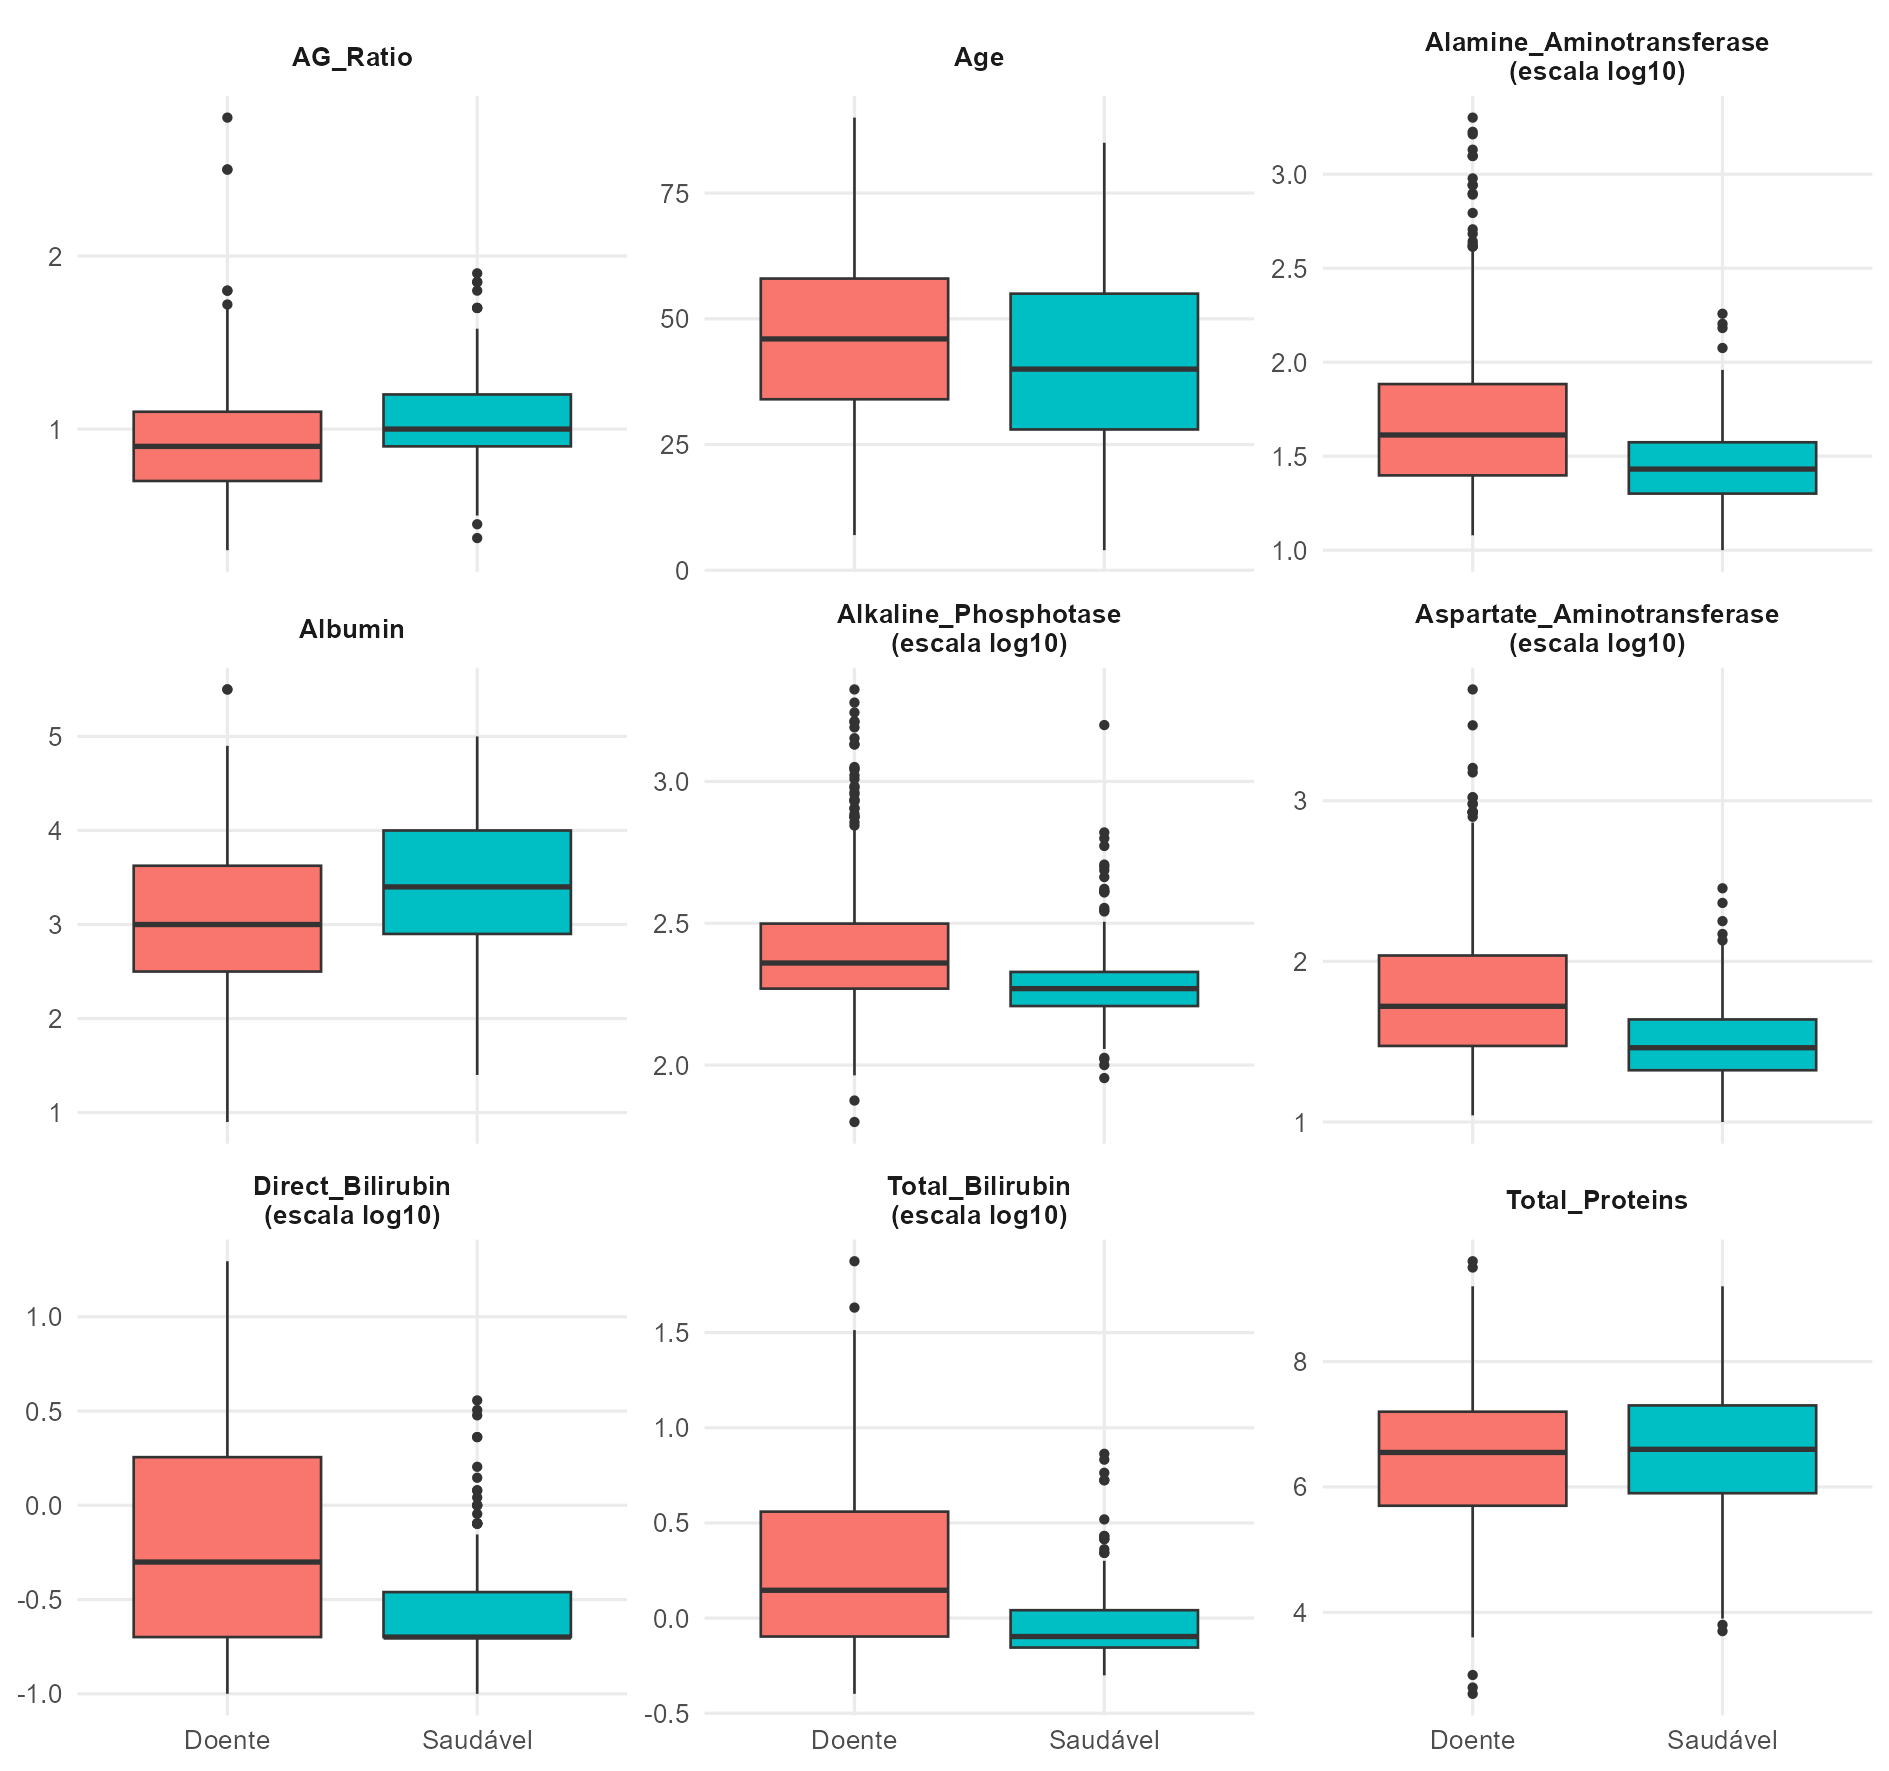
\includegraphics[width=\textwidth]{figuras/cap4-metodologia/eda_boxplots_por_classe.png}
\caption{Boxplots das variáveis numéricas, separados por classe (doente \textit{vs.} saudável).}
\label{fig:eda_boxplots}
\end{figure}

\subsection{Análise de Correlação}

Por fim, calculou-se a matriz de correlação de Pearson entre as variáveis numéricas 
(Figura~\ref{fig:eda_correlacao}). As observações com valores ausentes foram excluídas apenas para esse
cálculo. O objetivo foi identificar \textbf{multicolinearidade}, ou seja, pares de 
variáveis que carregam praticamente a mesma informação. Adotou-se $|r| > 0{,}7$ como 
limiar de correlação forte \cite{Dormann2012Collinearity, Mukaka2012Statistics}.

\begin{figure}[htbp]
\centering
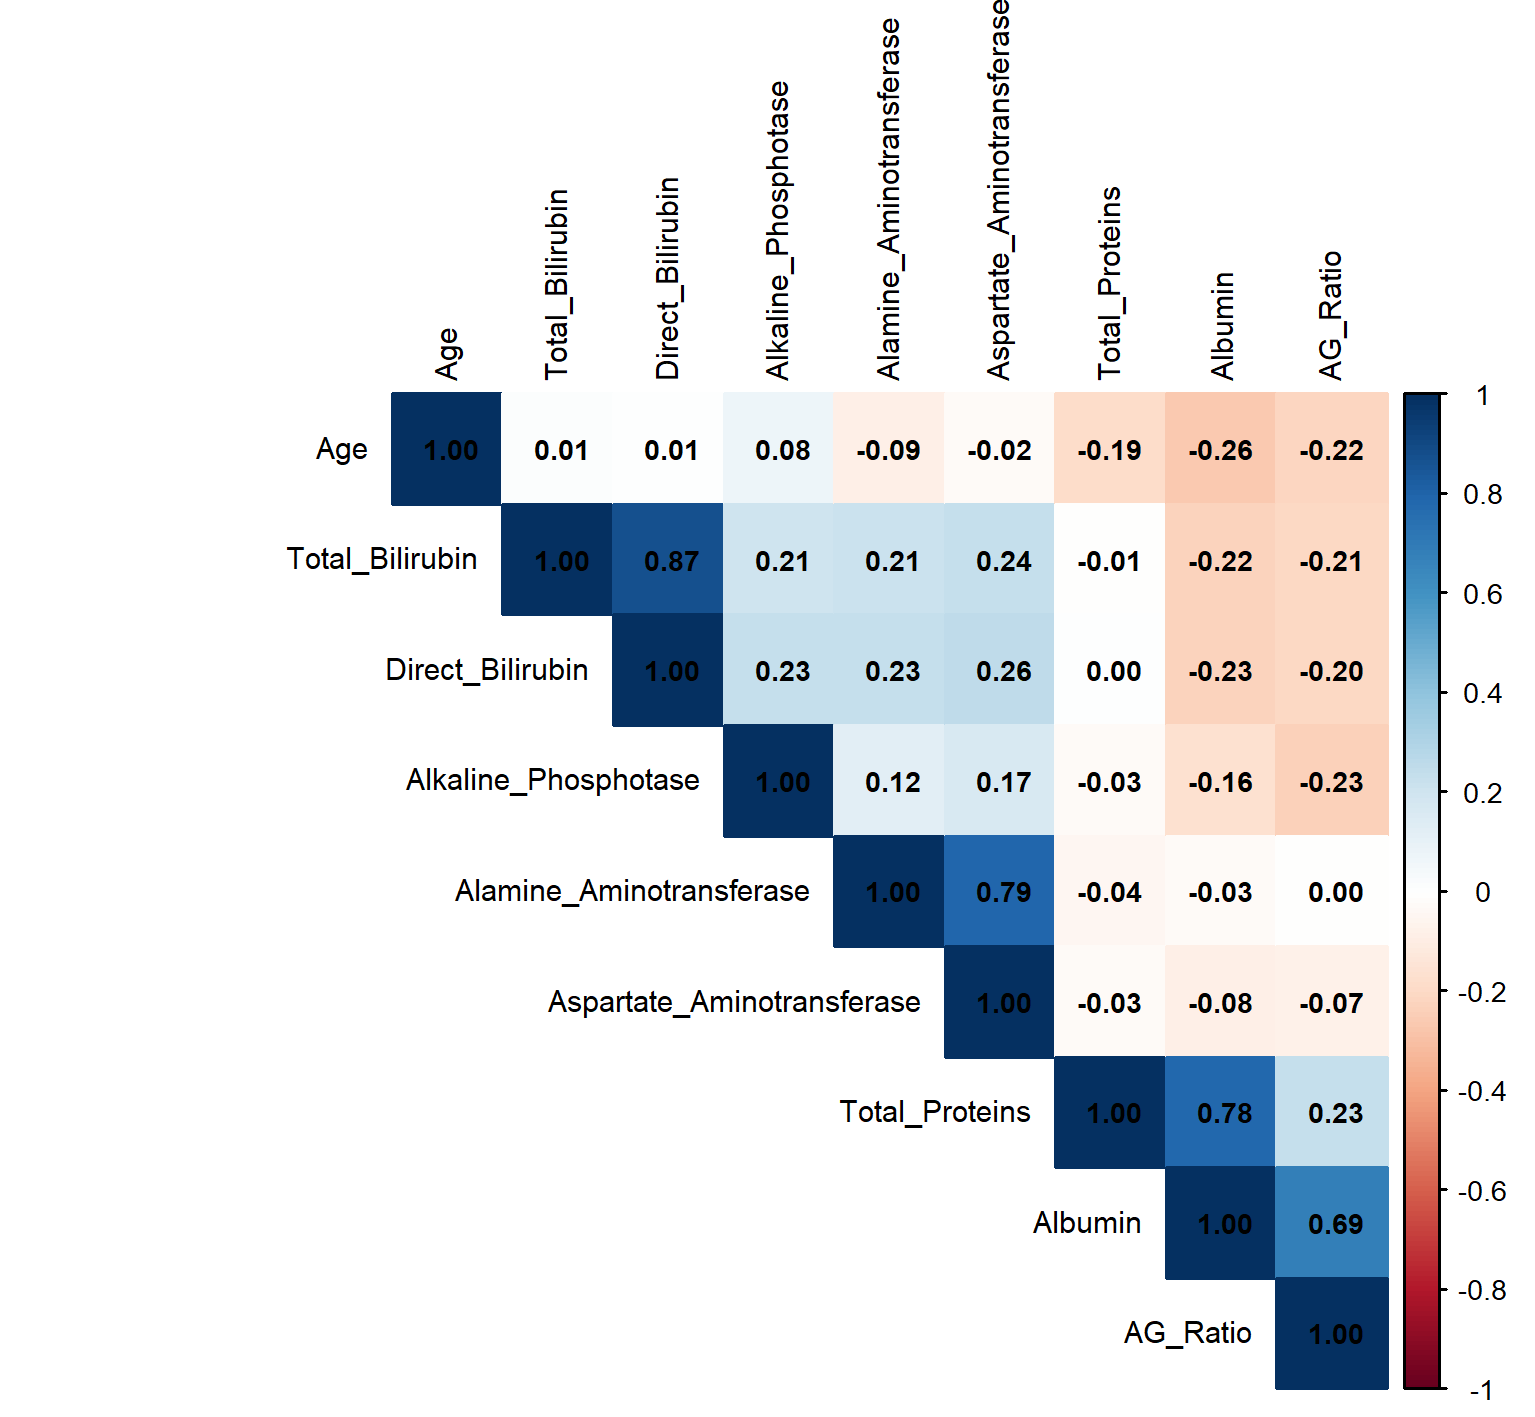
\includegraphics[width=0.8\textwidth]{figuras/cap4-metodologia/eda_correlacao.png}
\caption{Matriz de correlação de Pearson entre as variáveis numéricas.}
\label{fig:eda_correlacao}
\end{figure}

Encontrou-se correlação forte nos pares \textit{Total\_Bilirubin} × 
\textit{Direct\_Bilirubin} ($r = 0{,}874$), \textit{Alamine\_Aminotransferase} × 
\textit{Aspartate\_Aminotransferase} ($r = 0{,}792$) e \textit{Total\_Proteins} × 
\textit{Albumin} ($r = 0{,}783$). Essas correlações têm explicação fisiológica: 
a bilirrubina direta é uma das frações que compõem a bilirrubina total 
\cite{Fevery2008Bilirubin, Kwo2016ACG}, e a razão albumina/globulina é derivada 
da albumina e das proteínas totais, uma vez que a globulina é obtida pela 
diferença entre as duas \cite{Busher1990Albumin, Newsome2018Guidelines}.

Mesmo com essa redundância, optou-se por \textbf{manter todas as variáveis}. A decisão 
tem três motivos:
\begin{enumerate}
    \item Os modelos baseados em árvores (\textit{Random Forest}, XGBoost e LightGBM) 
    são, em geral, robustos à multicolinearidade quanto ao desempenho preditivo 
    \cite{Breiman2001RandomForests, Chen2016XGBoost, Ke2017LightGBM}. Em estudo de 
    simulação com diferentes níveis de colinearidade, \citeonline{Dormann2012Collinearity} 
    observaram que \textit{Random Forest} e árvores com \textit{boosting} mantiveram 
    desempenho estável em dados de teste, degradando apenas sob correlações extremas 
    ou quando a estrutura de correlação muda entre treino e teste, situação que não 
    se aplica a este trabalho, pois treino e teste provêm da mesma base;
    \item Excluir variáveis clinicamente relevantes contraria o objetivo de 
    interpretabilidade deste trabalho, que é entender como os modelos usam os exames 
    laboratoriais disponíveis;
    \item A multicolinearidade afeta principalmente a \textit{interpretação} dos 
    modelos, não sua capacidade preditiva \cite{Strobl2008Conditional, Dormann2012Collinearity}. 
    No caso do método SHAP, a presença de variáveis correlacionadas pode levar à 
    divisão da importância entre elas: como o modelo pode usar qualquer uma das 
    variáveis redundantes para capturar a mesma informação, o crédito atribuído a 
    cada uma individualmente tende a se diluir \cite{Aas2021Explaining, Chen2023Algorithms, Verdinelli2024Feature}. 
    Esse efeito é particularmente relevante na variante do TreeSHAP utilizada 
    neste trabalho para o XGBoost e o LightGBM, que estima as contribuições a 
    partir da estrutura das próprias árvores e das frequências de passagem pelos 
    nós, aproximando a distribuição condicional das variáveis 
    \cite{Lundberg2020Trees, Chen2023Algorithms}. Já para o \textit{Random Forest}, 
    cujos valores SHAP foram estimados por amostragem de Monte Carlo com permutação 
    marginal, as variáveis são tratadas como independentes, o que evita a divisão 
    de crédito mas pode avaliar o modelo em combinações de valores pouco plausíveis 
    quando há dependência \cite{Chen2020TrueToModel}. Essa diferença entre 
    estimadores é considerada explicitamente na discussão dos resultados.
\end{enumerate}

Como limitação, o coeficiente de Pearson mede apenas associações lineares e é 
sensível a valores extremos: um único ponto atípico pode alterar substancialmente a 
magnitude e até o sinal do coeficiente \cite{Schober2018Correlation}. 
Como as correlações foram calculadas na escala original, a presença de variáveis 
muito assimétricas pode ter influenciado a magnitude dos coeficientes, uma vez que 
distribuições com caudas pesadas tendem a inflar o valor de $r$ 
\cite{Bishara2015Reducing}.

\section{Pré-processamento}

\subsection{Remoção de Duplicatas}

Os 13 registros duplicados identificados na análise exploratória foram removidos, 
e a base passou de 583 para 570 registros.

\subsection{Transformação Logarítmica}

Às cinco variáveis assimétricas identificadas na análise exploratória aplicou-se a 
transformação $x' = \ln(1 + x)$ (Seção~\ref{sec:estatisticas_descritivas_assimetria}) \cite{logtransformation}. O logaritmo comprime a cauda da
distribuição sem alterar a ordem entre as observações: na 
\textit{Aspartate\_Aminotransferase}, por exemplo, o máximo, que era mais de 
cem vezes maior que a mediana na escala original, passa a ser cerca de duas 
vezes maior na escala transformada. Após a transformação, calculada sobre a 
base já sem os registros duplicados ($n = 570$), os coeficientes de 
assimetria passaram a variar entre 1,24 e 1,72, todos abaixo do limiar 
adotado (Tabela~\ref{tab:assimetria_log}). A soma de uma unidade antes do 
logaritmo garante que a transformação seja bem definida para valores 
próximos de zero, como os da \textit{Direct\_Bilirubin} (mínimo de 0,1 mg/dL).

Observe-se que os valores da coluna ``Antes'' da Tabela~\ref{tab:assimetria_log} 
diferem ligeiramente dos apresentados na Tabela~\ref{tab:descritivas}. A diferença 
não é um erro: a Tabela~\ref{tab:descritivas} descreve a base original completa 
($n = 583$), enquanto a Tabela~\ref{tab:assimetria_log} foi calculada após a 
remoção dos 13 registros duplicados ($n = 570$), que é a base efetivamente usada 
no pré-processamento. Como o coeficiente de assimetria é sensível à composição 
exata da amostra, a exclusão de poucas observações já produz pequenas variações 
nas casas decimais, sem alterar nenhuma das conclusões.

Cabe ainda um esclarecimento sobre o momento em que essa transformação é aplicada. 
Diferentemente da imputação pela mediana e da padronização, que dependem de 
parâmetros estimados a partir dos dados (mediana, média e desvio-padrão do 
treino), a transformação $\ln(1+x)$ é \textbf{determinística e livre de 
parâmetros}: o valor transformado de cada observação depende exclusivamente 
dela mesma, e não de nenhuma estatística do conjunto. Por isso, aplicá-la antes 
da divisão treino/teste, como foi feito neste trabalho, não introduz vazamento 
de dados, pois nenhuma informação do conjunto de teste é usada para definir a 
transformação \cite{KaufmanScharRosset2012}. O mesmo não valeria, por exemplo, 
para uma transformação de Box-Cox, cujo expoente $\lambda$ é estimado a partir 
dos dados e, portanto, deveria ser ajustado apenas no treino.

\begin{table}[htbp]
\centering
\caption{Coeficiente de assimetria ($b_1$) antes e depois da transformação $\ln(1+x)$ ($n = 570$).}
\label{tab:assimetria_log}
\begin{tabular}{lrr}
\hline
\textbf{Variável} & \textbf{Antes} & \textbf{Depois} \\
\hline
Total\_Bilirubin            & 4,84  & 1,72 \\
Direct\_Bilirubin           & 3,17  & 1,68 \\
Alkaline\_Phosphotase       & 3,71  & 1,32 \\
Alamine\_Aminotransferase   & 6,66  & 1,46 \\
Aspartate\_Aminotransferase & 10,50 & 1,24 \\
\hline
\end{tabular}
\end{table}

A transformação é especialmente relevante para a Regressão Logística, que 
assume relação linear entre os preditores e o logaritmo da razão de chances 
e é sensível a observações extremas \cite{Hosmer2005Applied}. Na escala logarítmica, o efeito 
de cada exame passa a depender de variações proporcionais, como dobrar o 
valor de uma enzima, o que é mais coerente com a interpretação clínica desses 
marcadores. Já os modelos baseados em árvores de decisão são, em princípio, 
invariantes a transformações monotônicas, pois suas divisões dependem apenas 
da ordem dos valores \cite{elementsofstatiscal}. Ainda assim, a transformação foi aplicada a 
todos os modelos, para que fossem comparados sobre a mesma representação dos 
dados, o que também facilita a leitura dos gráficos de dependência SHAP, nos 
quais os pacientes passam a se distribuir de forma mais uniforme ao longo do 
eixo horizontal.

\subsection{Divisão Treino/Teste}
\label{sec:divisao_treino_teste}

Após as transformações determinísticas, os dados foram divididos em conjuntos
de treino e teste na proporção de 80\% e 20\%, respectivamente, por meio da
função \texttt{createDataPartition} do pacote \texttt{caret}. A divisão foi
estratificada pela variável-alvo, preservando a proporção das classes em ambos
os conjuntos. Uma semente aleatória fixa, definida uma única vez no início do
\textit{pipeline}, garante a reprodutibilidade dessa partição. Essa divisão
ocorre antes da imputação e da padronização, de modo que os parâmetros dessas
duas etapas sejam estimados exclusivamente no conjunto de treino, evitando o
vazamento de informação do conjunto de teste \cite{KaufmanScharRosset2012}.

\subsection{Imputação de Valores Ausentes}

A mediana foi calculada exclusivamente no conjunto de treino e depois aplicada a 
ambos os conjuntos (Seção~\ref{sec:divisao_treino_teste}).

\subsection{Padronização}
\label{sec:padronizacao}

Após a imputação, os preditores foram padronizados pela transformação
\textit{z-score}, com centralização (\textit{center}) e escalonamento
(\textit{scale}). As médias e os desvios-padrão foram estimados exclusivamente
no conjunto de treino e, em seguida, aplicados tanto ao treino quanto ao teste,
mantendo a separação entre os dados usados para ajustar os parâmetros e os
usados para avaliação. Essa etapa é particularmente relevante para a Regressão
Logística, um modelo linear sensível às escalas dos preditores; para os modelos
baseados em árvores, que realizam divisões pela ordem dos valores, a
padronização tende a ser menos relevante.

\subsection{Balanceamento de Classes (SMOTE)}
\label{sec:balanceamento}

Para lidar com o desbalanceamento das classes, utilizou-se o SMOTE
(\textit{Synthetic Minority Over-sampling Technique})\cite{smote}, que gera amostras
sintéticas da classe minoritária a partir de observações existentes. O
balanceamento é aplicado somente aos dados de treino; o conjunto de teste
mantém sua distribuição original e nunca é balanceado. Durante o treinamento
com validação cruzada, o SMOTE é aplicado independentemente dentro de cada
partição de treino de cada \textit{fold}, após a separação dos \textit{folds}.
Assim, as amostras sintéticas não contaminam as partições de validação — o que
poderia ocorrer se o balanceamento fosse feito antes da divisão — nem inflacionam
artificialmente as métricas de desempenho.

\section{Modelos Preditivos}

Foram comparados quatro classificadores com diferentes graus de flexibilidade:
um modelo linear, empregado como referência interpretável, e três métodos
baseados em árvores, capazes de representar relações não lineares e interações
entre os preditores. Essa comparação permite examinar se a maior flexibilidade
dos modelos de conjunto oferece vantagens preditivas em relação a uma
abordagem linear, sem pressupor de antemão qual método terá o melhor
desempenho. A classe positiva considerada no treinamento é ``doente''.

\subsection{Regressão Logística}

A Regressão Logística modela a probabilidade de pertencimento à classe positiva
por meio da função logística aplicada a uma combinação linear dos preditores.
Embora seja um classificador linear na escala dos logitos, a transformação
logística produz probabilidades entre zero e um. Seus coeficientes descrevem
a variação nos logitos associada aos preditores, mantidos os demais constantes;
a exponenciação de cada coeficiente fornece a correspondente razão de chances
(\textit{odds ratio}) \cite{Hosmer2005Applied, elementsofstatiscal}.

Neste estudo, ajustou-se o modelo binomial sem busca de hiperparâmetros. Ele foi
incluído como \textit{baseline} por combinar uma formulação estatística
conhecida com interpretação direta dos coeficientes, oferecendo um ponto de
comparação para os métodos de árvores. Como os preditores numéricos foram
padronizados, os coeficientes correspondem a variações de uma unidade na escala
padronizada; suas exponenciais são apresentadas como razões de chances.

\subsection{Random Forest}

O Random Forest constrói um conjunto de árvores de decisão a partir de
reamostragens dos dados e de subconjuntos aleatórios de preditores considerados
nas divisões. Para classificação, as árvores contribuem para a previsão
agregada do conjunto. A aleatorização e a agregação visam reduzir a variância
em relação a uma árvore individual, preservando a capacidade de representar
relações não lineares \cite{Breiman2001RandomForests}.

Esse método foi incluído por oferecer uma estratégia de \textit{bagging}
robusta e não linear, distinta do ajuste aditivo por boosting dos outros
métodos de árvores. No treinamento, foram utilizadas 500 árvores; os demais
parâmetros considerados pelo classificador foram selecionados no procedimento
de busca descrito na seção seguinte.

\subsection{XGBoost}

O XGBoost é um método de \textit{gradient boosting} que constrói árvores
sequencialmente: cada nova etapa busca reduzir a função de perda, levando em
conta os erros do conjunto de árvores já ajustado. A implementação acrescenta
recursos de regularização e eficiência computacional ao processo de
aprendizado de árvores \cite{Chen2016XGBoost}.

Sua inclusão permite avaliar uma abordagem de boosting amplamente utilizada,
com mecanismos de regularização e uma implementação otimizada, em contraste
com a agregação por reamostragem do Random Forest. Os parâmetros da variante
de árvores do XGBoost foram selecionados por busca aleatória, conforme o
protocolo de treinamento.

\subsection{LightGBM}

O LightGBM é outro método de \textit{gradient boosting} baseado em árvores,
projetado para treinar de forma eficiente em conjuntos de dados de maior
dimensão. Sua estratégia de crescimento das árvores e suas técnicas de
amostragem e representação de atributos buscam reduzir o custo computacional
sem abandonar o ajuste sequencial característico do boosting
\cite{Ke2017LightGBM}.

O método foi incluído para comparar uma implementação de boosting com
estratégia de eficiência distinta à do XGBoost. Como o ambiente de treinamento
utilizado não oferece suporte nativo ao LightGBM, a integração foi feita por
meio de um adaptador compatível com a interface de treinamento empregada no
pipeline; seus hiperparâmetros foram submetidos à mesma busca aleatória dos
demais modelos ajustáveis.

\section{Treinamento e Validação Cruzada}

O treinamento e a seleção de modelos foram conduzidos apenas com o conjunto de
treino, preservando o conjunto de teste separado para a avaliação final. Para
estimar o desempenho durante o desenvolvimento, utilizou-se validação cruzada
repetida, com cinco partições (\textit{folds}) e três repetições. Em cada
rodada, quatro partições são usadas para ajuste e a partição restante para
validação; as repetições submetem os modelos a partições distintas e reduzem
a dependência dos resultados em relação a uma única divisão aleatória dos
dados.

Nos modelos que possuem parâmetros de ajuste, foram avaliadas 30 combinações
amostradas por busca aleatória. Em comparação com uma grade exaustiva, a busca
aleatória permite explorar valores distintos em cada dimensão do espaço de
hiperparâmetros, sem exigir a avaliação de todas as combinações cartesianas;
essa abordagem é particularmente útil quando apenas parte dos parâmetros
influencia fortemente o desempenho \cite{}% TODO: buscar Bergstra e Bengio (2012), “Random Search for Hyper-Parameter Optimization”. Prompt para Consensus: “Qual é o artigo de Bergstra e Bengio, publicado em 2012, que compara busca aleatória e busca em grade para otimização de hiperparâmetros, e quais são seus principais argumentos de eficiência?”
A Regressão Logística, ajustada sem hiperparâmetros a otimizar, não requer essa
busca.

A seleção dos modelos e das combinações de hiperparâmetros foi baseada na área
sob a curva ROC (AUC-ROC), calculada a partir das probabilidades estimadas para
a classe positiva. A AUC resume a capacidade de ordenação dos casos positivos
acima dos negativos ao longo dos limiares, sem depender de um único ponto de
corte. Por isso, complementa a acurácia, que pode ser enganosa quando as
classes têm frequências diferentes: como discutido na Análise Exploratória,
um classificador pode obter acurácia aparentemente alta favorecendo a classe
mais frequente sem discriminar adequadamente os casos da classe minoritária
\cite{FAWCETT2006861, imbalancedata}.

O desbalanceamento foi tratado dentro do procedimento de reamostragem: em cada
\textit{fold}, o SMOTE é aplicado somente à partição usada para ajustar o
modelo, depois da separação da partição de validação. Dessa forma, as
observações sintéticas não são compartilhadas com a validação, evitando
vazamento de informação e mantendo a estimativa de desempenho baseada em dados
não balanceados artificialmente.

Ao final da validação cruzada, os resultados dos quatro modelos foram
comparados pela distribuição das AUCs nos \textit{folds}, apresentada em
gráfico de caixas, e por testes t pareados com correção de Bonferroni para as
comparações entre pares. A comparação pareada considera que os modelos foram
avaliados nas mesmas partições; a correção de Bonferroni controla o aumento do
erro tipo I decorrente das comparações múltiplas. A literatura sobre
comparação estatística de classificadores discute as escolhas e limitações
desses procedimentos \cite{}% TODO: buscar Janez Demšar (2006), “Statistical Comparisons of Classifiers over Multiple Data Sets”. Prompt para Consensus: “Quais procedimentos estatísticos Demšar recomenda em 2006 para comparar classificadores e quais são as limitações de testes pareados sobre resultados de validação cruzada?”

\section{Avaliação de Desempenho}

Após a seleção e o ajuste dos modelos, o desempenho foi medido no conjunto de
teste, que não participou do treinamento, da seleção de hiperparâmetros nem da
geração de amostras SMOTE. Esse conjunto manteve a distribuição observada das
classes, de modo que as métricas finais reflitam a prevalência original dos
dados e não uma distribuição artificialmente balanceada. Para cada modelo,
foram obtidas as previsões de classe e as probabilidades estimadas para
``doente''.

A matriz de confusão resume verdadeiros positivos, verdadeiros negativos,
falsos positivos e falsos negativos para um limiar de decisão. No limiar padrão
de 0,5, a partir dela foram calculadas a acurácia, a acurácia balanceada, a
sensibilidade, a especificidade, a precisão, a medida F1 e a estatística Kappa;
a AUC-ROC foi calculada a partir das probabilidades. A sensibilidade corresponde à
proporção de doentes identificados, enquanto a especificidade corresponde à
proporção de não doentes identificados. A precisão expressa a proporção de
previsões positivas que são de fato positivas, e a medida F1 resume o
equilíbrio entre precisão e sensibilidade. A acurácia balanceada dá peso
igual à sensibilidade e à especificidade, e o Kappa expressa a concordância
entre classe prevista e observada descontada a concordância esperada ao acaso.
Para a AUC de cada modelo, foram calculados intervalos de confiança de 95\%
pelo método de DeLong.

Considerar a acurácia isoladamente seria inadequado diante do desbalanceamento
identificado na AED: ela pode ser dominada pelo desempenho na classe mais
frequente e ocultar erros na classe minoritária. Por essa razão, a avaliação
considera conjuntamente métricas por classe, acurácia balanceada e AUC, em
consonância com a discussão sobre curvas ROC e classificação em bases
desbalanceadas \cite{FAWCETT2006861, imbalancedata}. Também foram construídas
curvas Precision--Recall. Como elas relacionam precisão e sensibilidade da
classe positiva, complementam a curva ROC ao tornar explícito o compromisso
entre encontrar casos doentes e limitar os falsos positivos em um cenário no
qual a prevalência da classe positiva não é majoritária.

Além do limiar padrão de 0,5, foram examinados dois critérios de decisão. O
primeiro é o limiar que maximiza o índice de Youden, definido pela soma da
sensibilidade e da especificidade menos um. O segundo é um limiar clínico
escolhido para garantir sensibilidade de pelo menos 90\%, selecionando, entre
os limiares que atendem a essa meta, aquele que preserva a maior especificidade
possível. Essa análise prioriza a redução de falsos negativos — pacientes
doentes classificados como não doentes —, erro considerado especialmente
crítico em um cenário de triagem clínica, no qual um resultado negativo
equivocado pode atrasar a investigação diagnóstica \cite{}% TODO: buscar literatura de diagnóstico médico sobre custo assimétrico de falsos negativos e priorização de sensibilidade em triagem. Prompt para Consensus: “Que estudos ou diretrizes de diagnóstico clínico discutem o custo de falsos negativos e justificam priorizar alta sensibilidade em testes de triagem médica?”

As AUCs dos quatro modelos no conjunto de teste também foram comparadas em
pares pelo teste de DeLong para curvas ROC. O método permite avaliar a
diferença entre áreas sem tratar as estimativas das curvas como independentes
quando são obtidas nos mesmos pacientes \cite{}% TODO: buscar Elizabeth R. DeLong, David M. DeLong e Daniel L. Clarke-Pearson (1988), “Comparing the Areas under Two or More Correlated Receiver Operating Characteristic Curves: A Nonparametric Approach”. Prompt para Consensus: “Qual método não paramétrico DeLong, DeLong e Clarke-Pearson propuseram em 1988 para comparar as áreas sob duas ou mais curvas ROC correlacionadas?”

Por fim, as métricas foram calculadas separadamente para pacientes do sexo
feminino e masculino, como continuação da preocupação com a predominância
masculina observada na AED. Para cada grupo foram estimadas AUC e seu intervalo
de confiança de 95\%, sensibilidade e especificidade. A diferença de AUC entre
os grupos foi avaliada pelo teste de DeLong para amostras independentes, e
também foram examinadas as diferenças de sensibilidade e especificidade. Essa
estratificação permite identificar possíveis disparidades de desempenho e
risco desigual de falsos negativos, sem, por si só, estabelecer sua causa;
essa auditoria é relevante diante das preocupações com viés algorítmico em
saúde \cite{Rajkomar2018Ensuring, investigatingbiashealth}. As diferenças
devem ser interpretadas com cautela, considerando a quantidade de observações
disponíveis em cada grupo.

\section{Interpretabilidade com SHAP}

Os valores SHAP (\textit{SHapley Additive exPlanations}) adaptam os valores de
Shapley da teoria dos jogos cooperativos para atribuir a cada preditor uma
contribuição à previsão de um modelo. Para uma observação, cada contribuição
representa a parcela associada à variável na diferença entre uma previsão de
referência e a previsão obtida para aquela observação, segundo a definição do
valor de Shapley. Essa formulação fornece explicações locais aditivas, que
podem também ser agregadas para descrever padrões globais \cite{}% TODO: buscar Scott M. Lundberg e Su-In Lee (2017), “A Unified Approach to Interpreting Model Predictions”, artigo original que introduziu SHAP. Prompt para Consensus: “Qual artigo de Lundberg e Lee, publicado em 2017, introduziu SHAP como uma abordagem unificada para interpretar previsões de modelos de machine learning?”

O cálculo depende do tipo de modelo. Para XGBoost e LightGBM, foram usados
valores TreeSHAP exatos, obtidos pelas contribuições nativas das árvores. No
fluxo adotado, essas contribuições estão na escala de logitos (\textit{log-odds});
valores positivos deslocam a previsão em direção à classe ``doente'' e valores
negativos em direção à classe ``saudável''. TreeSHAP permite calcular as
atribuições para modelos de árvores explorando sua estrutura
\cite{Lundberg2020Trees}.

Para o Random Forest, utilizou-se o pacote \textit{fastshap} para obter uma
estimativa amostral de SHAP por Monte Carlo, com 100 simulações por explicação
e na escala de probabilidade. Essa
escolha decorre de o fluxo utilizado não dispor de TreeSHAP exato para o
Random Forest. A estimativa amostral aproxima as contribuições a partir de
coalizões de variáveis; diferentemente do cálculo TreeSHAP empregado para os
modelos de boosting, o procedimento adotado trata as variáveis como
independentes ao construir as amostras de referência. As diferenças de
algoritmo e de escala devem ser consideradas ao interpretar e comparar os
valores obtidos \cite{}% TODO: buscar o trabalho original sobre Kernel SHAP e amostragem de valores de Shapley, associado a Scott M. Lundberg e Su-In Lee (2017), “A Unified Approach to Interpreting Model Predictions”, e verificar a formulação de Shapley Sampling Values. Prompt para Consensus: “Qual publicação original descreve Kernel SHAP e a aproximação amostral dos valores de Shapley para explicar previsões de modelos, e como o método amostra coalizões de variáveis?”

Os coeficientes e respectivas razões de chances da Regressão Logística
fornecem uma representação direta dos efeitos estimados, de modo que esse
modelo não integra a seleção padrão de modelos a explicar. A regra também
inclui o melhor modelo no teste segundo a AUC; caso a Regressão Logística
ocupe essa posição, ela é incluída nessa seleção. Assim, são explicados o
XGBoost, o Random Forest e o melhor modelo no teste, removendo-se duplicatas.

Para cada modelo explicado, a importância global de uma variável é calculada
pela média do valor absoluto de SHAP entre os pacientes; ela resume a
magnitude média da contribuição, mas não informa sua direção. O gráfico
\textit{beeswarm} mostra a distribuição das contribuições individuais e
relaciona sua posição com os valores das variáveis, permitindo observar
heterogeneidade entre pacientes. A direção do efeito também é examinada pela
correlação entre o valor de cada variável e seu valor SHAP; essa associação é
descritiva e não deve ser interpretada como efeito causal. Para as quatro
variáveis de maior importância, gráficos de dependência mostram como as
contribuições variam ao longo dos valores observados. Por fim, gráficos
\textit{waterfall} decompõem previsões individuais em relação ao valor de
referência, mostrando como as contribuições de cada variável conduzem à
previsão do paciente.

As explicações locais são produzidas para três casos definidos a partir do
conjunto de teste: o verdadeiro positivo com maior probabilidade estimada de
doença, o verdadeiro negativo com menor probabilidade estimada de doença e o
falso negativo de pior erro, isto é, o paciente doente com menor probabilidade
estimada de pertencer à classe positiva. A seleção torna possível examinar
tanto previsões corretas de maior confiança quanto um caso particularmente
crítico de doença não identificada.

Como aprofundamento da avaliação de desempenho por sexo, a importância SHAP
também é calculada separadamente para os grupos feminino e masculino. A
concordância entre os rankings de importância de cada grupo é resumida pela
correlação de Spearman; adicionalmente, examina-se a contribuição SHAP média
com sinal da variável \textit{Gender} em cada grupo. Essas análises descrevem
se o modelo distribui e direciona suas contribuições de modo semelhante
entre os grupos, sem substituir a avaliação de disparidades de desempenho nem
permitir, isoladamente, inferências causais.

Por último, os rankings de importância são comparados entre os quatro
classificadores. Para XGBoost e Random Forest são consideradas as importâncias
SHAP; para Random Forest e LightGBM também se obtêm importâncias nativas dos
modelos, e para a Regressão Logística usa-se o valor absoluto dos coeficientes
padronizados. A concordância entre esses rankings é examinada por correlação
de Spearman. Como as medidas de importância têm definições e escalas
diferentes, a comparação enfatiza a ordenação relativa das variáveis, e não a
equivalência numérica das contribuições.
